\documentclass{beamer}
\usepackage[utf8]{inputenc}
\usepackage{natbib}
\usepackage{graphicx}
\usepackage{hyperref}

\title{Edwin Catmull}
\subtitle{By William Vida}
\date{}

\begin{document}

\frame {
	\titlepage
}

\frame{
	\begin{figure}[htp]
		\centering
		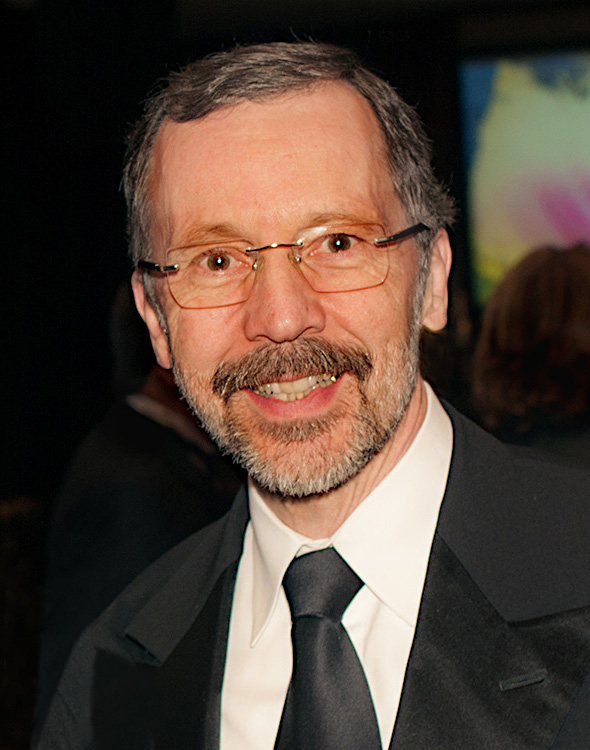
\includegraphics[width=6cm]{images/Edwin Catmull.jpg}
	\end{figure}
}

\frame{
	\frametitle{Introduction}
	\begin{itemize}
		\item Edwin Catmull is an American computer scientist known for his great contributions towards 3D computer graphics.
		\item Catmull was one of the founders of Pixar Animation Studios. 
		\item Catmull was one of the developers of Pixar's RenderMan rendering software.
		\item He was awarded the 2019 A.M. Turing award along with Pat Hanrahan for their "fundamental contributions to 3-D computer graphics, and the revolutionary impact of these techniques on computer-generated imagery (CGI) in filmmaking and other applications".
	\end{itemize}
}
	
\frame{
	\frametitle{Examples of Catmull's Contributions}
	\begin{itemize}
		\item Image compositing.
		\item Motion blur.
		\item Subdivision surfaces.
		\item Cloth simulation and rendering techniques.
		\item Texture mapping.
		\item Z-buffer.
		\item Bicubic patches.
	\end{itemize}
}

\frame{
	\frametitle{A Computer Animated Hand}
	\begin{itemize}
		\item A Computer Animated Hand is a 1972 computer-animated short film produced by Edwin Catmull and Fred Parke as a graduate student project.
		\item Catmull animated a human hand and it was one of the earliest examples of 3D computer animation.
		\item It is one minute long and it shows an animated hand turning, opening, closing, pointing and flexing its fingers.
		\item It was a revolutionary invention and Catmull worked out concepts that become the foundation for computer graphics following its completion.
		\item In 2011, it was introduced into the National Film Registry of the United States.
	\end{itemize}
}

\frame{
	\frametitle{A Computer Animated Hand}
	\begin{figure}[htp]
		\centering
		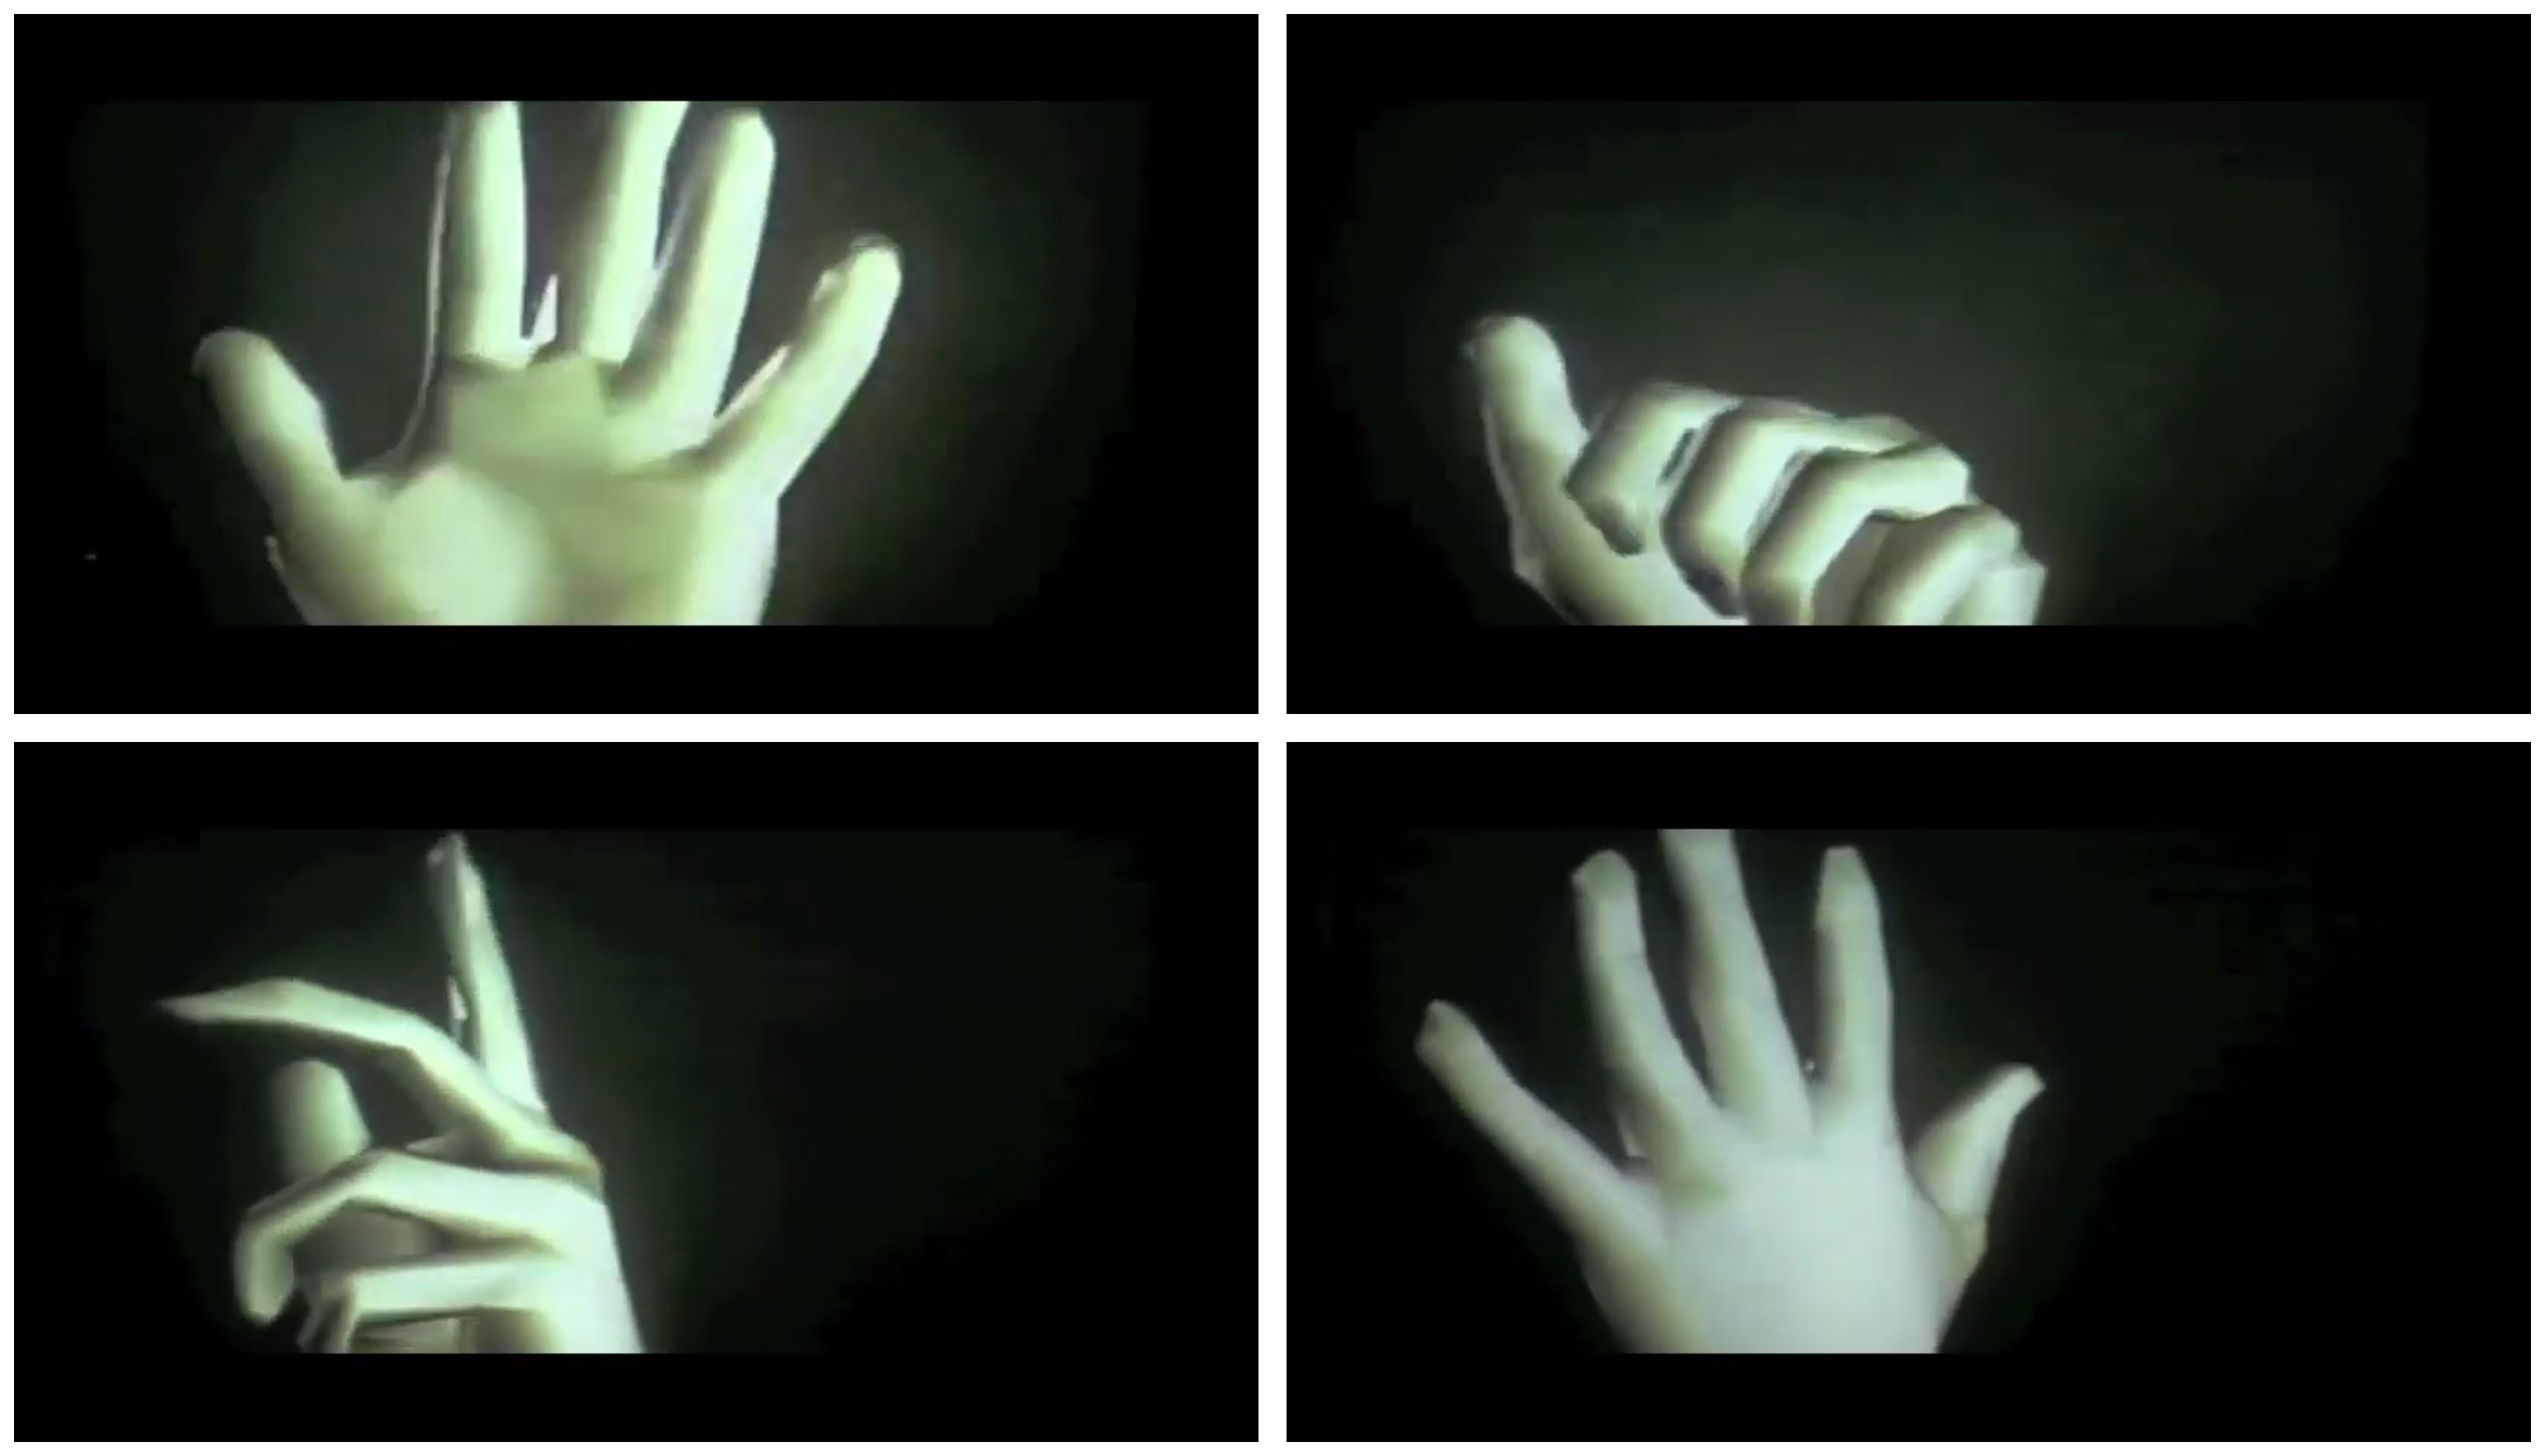
\includegraphics[width=10.5cm]{images/A Computer Animated Hand.jpg}
	\end{figure}
}

\frame{
	\frametitle{RenderMan}
	\begin{itemize}
		\item RenderMan is a piece of software that Pixar uses to create 3D animations. RenderMan has been used to create movies such as Toy Story, Independence Day, Monsters, Inc. and The Lion King.
		\item RenderMan incorporates some of Catmull's inventions such as z-buffering and subdivision surface algorithms.
	\end{itemize}
}

\frame{
	\frametitle{Texture Mapping}
	\begin{itemize}
		\item Catmull first described the process of texture mapping in his 1974 PhD thesis "A subdivision algorithm for computer display of curved surfaces".
		\item Texture mapping is a process in which a 2D surface is wrapped around a 3D object.
		\item Before Catmull's discovery, objects could only be set to one specific colour and adding detail became a much longer process.
		\item Catmull's original technique for texture mapping is referred to as diffuse mapping.
	\end{itemize}
}

\frame{
	\frametitle{Texture Mapping}
	\begin{figure}[htp]
		\centering
		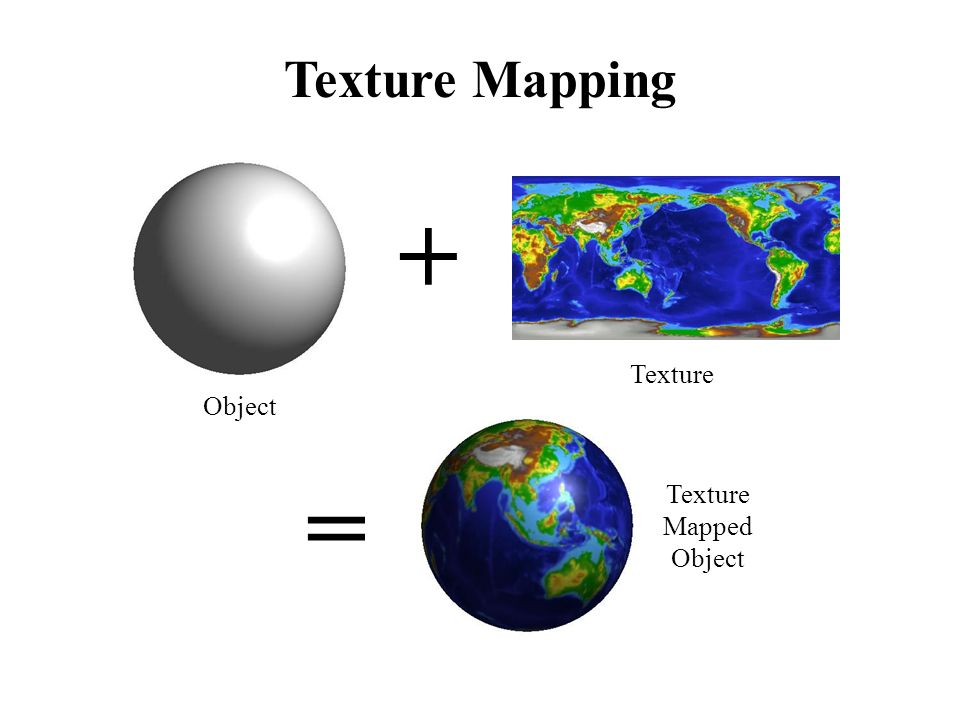
\includegraphics[width=10cm]{images/Texture Mapping.jpg}
	\end{figure}
}

\frame{
	\frametitle{Z-Buffering}
	\begin{itemize}
		\item Catmull is credited with the invention of the z-buffering concept.
		\item Z-buffering is a technique used in 3D computer graphics to determine what parts of an object are visible in a scene.
		\item The z-buffering algorithm uses the graphics processor to store each pixel's z-axis value in a special memory region called the Z-buffer. Different objects might have the same values for their x and y-coordinates, but have different values for their z-coordinates. The object with the lowest z-coordinate value is positioned in front of the other objects and that is the one that will be seen.
	\end{itemize}
}

\frame{
	\frametitle{Z-Buffering}
	Pseudocode of the algorithm:\\
	~\\
	{\small
		First of all, initialize the depth of each pixel.\\
		i.e,  d(i, j) = infinite (max length)\\
		Initialize the colour value for each pixel \\
		as c(i, j) = background colour\\
		for each polygon, do the following steps:\\
		~\\
		for (each pixel in polygon's projection)\\
		\{\\
		\qquad find depth i.e, z of polygon\\
		\qquad at (x, y) corresponding to pixel (i, j)\\
		~\\
		\qquad if (z $<$ d(i, j))\\
		\qquad \{\\
		\qquad \qquad d(i, j) = z;\\
		\qquad \qquad c(i, j) = colour;\\
		\qquad \}\\
		\}
	}
}

\frame{
	\frametitle{Z-Buffering}
	\begin{figure}[htp]
		\centering
		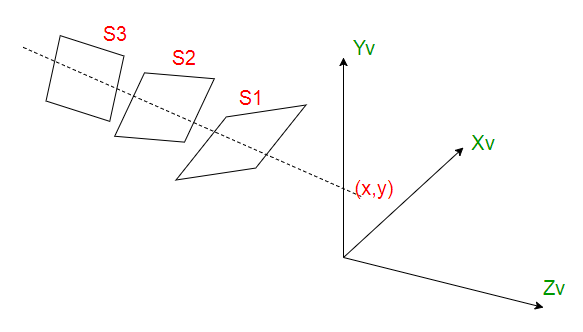
\includegraphics[width=10cm]{images/zbuffer.png}
	\end{figure}
	After the algorithm checks S1, S2 and S3, S1 will be visible from the viewpoint.
}

\frame{
	\frametitle{Z-Buffering}
	\begin{figure}[htp]
		\centering
		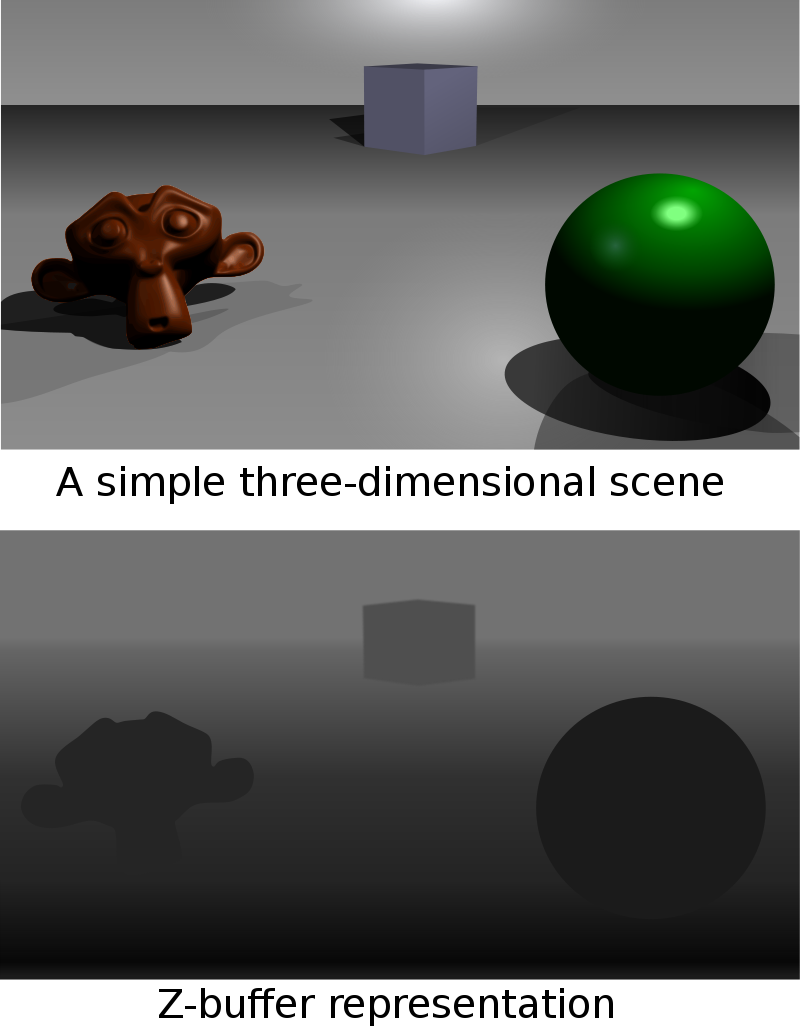
\includegraphics[width=6cm]{images/z-buffering-computer-model.png}
	\end{figure}
}

\frame{
	\frametitle{Subdivision Surface}
	\begin{itemize}
		\item Edwin Catmull and Jim Clark came up with the Catmull–Clark algorithm in 1978.
		\item The Catmull-Clark subdivision is a technique for smoothing the surface of a 3D polygon mesh by dividing the polygons of the surface into smaller polygons and repositioning the previous vertices based on vertices close to it. This approach takes each original polygon found in the mesh and divides the polygon into quadrilaterals (four-sided polygons) and then, based on the averages, constructs new vertices. After, it changes the original polygon's previous vertices depending on the surrounding area.
		\item It is a fast and effective algorithm.
	\end{itemize}
}

\frame{
	\frametitle{Subdivision Surface}
	\begin{figure}[htp]
		\centering
		\includegraphics[width=10cm]{images/Catmull–Clark.png}
		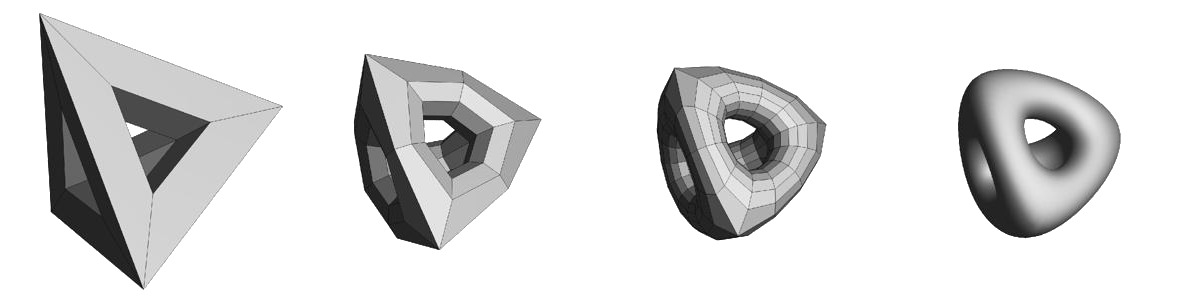
\includegraphics[width=10cm]{images/Catmull-Clark-2.jpg}
	\end{figure}
}

\frame{
	\frametitle{Spatial Anti-Aliasing}
	\begin{itemize}
		\item In 1978, Catmull released his thesis on spatial anti-aliasing titled "A hidden-surface algorithm with anti-aliasing".
		\item Aliasing happens when smooth and curved lines become rasterised and anti-aliasing is the process of the smoothening of the jagged edges.
		\item Anti-aliasing smoothes the pixels by filling in the jagged edges with shadowing pixels.
	\end{itemize}
}

\frame{
	\frametitle{Spatial Anti-Aliasing}
	\begin{figure}[htp]
		\centering
		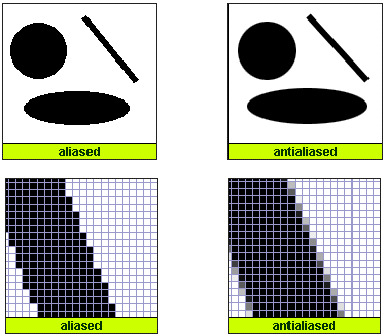
\includegraphics[width=8cm]{images/Spatial Anti-Aliasing.jpg}
	\end{figure}
}

\frame{
	\frametitle{Alpha Channel}
	\begin{itemize}
		\item Edwin Catmull and Alvy Ray Smith invented the concept of the alpha channel in RGBA.
		\item The alpha channel is used to make it seem that an image is partially to fully transparent compared to another image.
		\item Before the alpha channel, an image had to be rendered with different backgrounds which was a slow procedure. They came up with the idea when Catmull said that it would be easier to render the opacity with the colour information in a file for each pixel. Then the file could be made without rerendering over different backgrounds.
	\end{itemize}
}

\frame{
	\frametitle{Alpha Channel}
	\begin{figure}[htp]
		\centering
		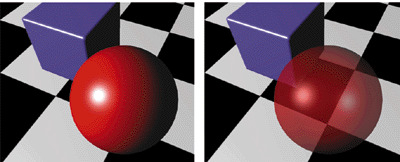
\includegraphics[width=10cm]{images/Alpha Channel.jpg}
	\end{figure}
}

\frame{
	\frametitle{Motion Blur}
	\begin{itemize}
		\item Motion blur is the streaking or tails of an object or objects when a picture or video is taken.
		\item Catmull wanted to recreate this in animations to add realism to animation scenes. Catmull said that solving this was the "single hardest problem we had".
		\item Rob Cook suggested looking at 16 pixel points at 1/60 of second (which is the speed at which a camera shutter opens and closes). Then, several different objects will move over that pixel. Tom Porter's answer was to get the colour of each of those 16 points at that moment. This allowed him to assign each pixel an average and this allowed a blurring effect to be reproduced in animations.
		\item Before this discovery, animation objects would move in a way where it seemed they were teleporting each time they moved.
	\end{itemize}
}

\frame{
	\frametitle{Motion Blur}
	\begin{figure}[htp]
		\centering
		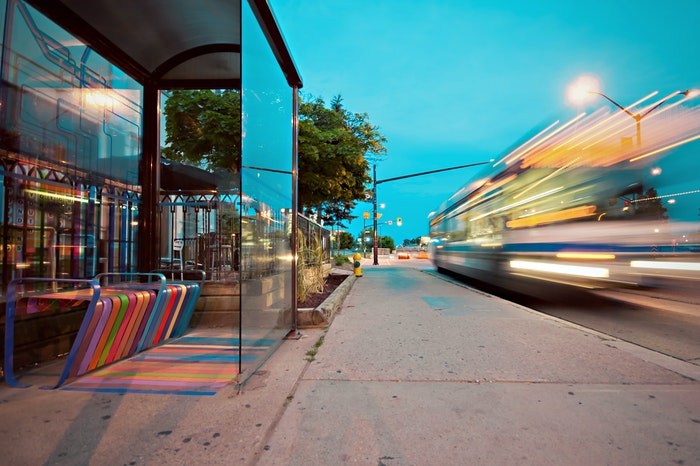
\includegraphics[width=10cm]{images/Motion blur.jpg}
	\end{figure}
}

\frame{
	\frametitle{Awards}
	\begin{itemize}
		\item Catmull has been awarded 5 Academy Awards, an IEEE John von Neumann Medal, the 2019 Turing Award, a Scientific and Engineering Award, an ACM SIGGRAPH Steven A. Coons Award and a Gordon E. Sawyer Award.
	\end{itemize}
}

\frame{
	\frametitle{References}
	\href{https://www.webopedia.com/definitions/z-buffering/}{Z-Buffering}
		
	\href{https://www.cs.utexas.edu/users/fussell/courses/cs384g-fall2011/lectures/lecture20-Z_buffer_pipeline.pdf}{Projections and Z-buffers}
		
	\href{https://www.geeksforgeeks.org/z-buffer-depth-buffer-method/}{Z-Buffer or Depth-Buffer method}
		
	\href{https://www.algosome.com/articles/catmull-clark-subdivision-algorithm.html}{3-DIMENSIONAL SMOOTHING: CATMULL-CLARK SUBDIVISION}
		
	\href{https://www.diva-portal.org/smash/get/diva2:945618/FULLTEXT02.pdf}{Proposed workflow for UV mapping and
	texture painting}
		
	\href{https://disney.fandom.com/wiki/Ed_Catmull}{Ed Catmull}
		
	\href{https://awards.acm.org/about/2019-turing}{2019 Turing Award}
		
	\href{https://www.computer.org/profiles/edwin-catmull}{Edwin Catmull}
		
	\href{https://www.geeksforgeeks.org/computer-graphics-antialiasing/}{Computer Graphics | Antialiasing}
		
	\href{https://www.anandtech.com/show/350/2}{3dfx T-Buffer Technology Overview}
		
	\href{https://computerhistory.org/profile/edwin-catmull/}{EDWIN CATMULL}
		
	\href{http://alvyray.com/Awards/AwardsAcademy96.htm}{The Alpha Channel}
		
	\href{https://www.cs.princeton.edu/courses/archive/spring05/cos426/papers/smith95c.pdf}{Alpha and the History of Digital Compositing}
		
	\href{http://parisinnovationreview.com/author/ed-catmull}{ED CATMULL}
		
	\href{https://spectrum.ieee.org/at-work/tech-careers/and-the-oscar-goes-to}{And the Oscar Goes To...}
		
	\href{https://stanfordmag.org/contents/paving-the-way}{Paving the Way}
}

\end{document}
